\section{Necessary \& Sufficient Conditions for Minimality}

This section explores some necessary and sufficient conditions for a query to be "minimal".
We start with some necessary definitions.
\AP
We say that a (U)CRPQ is \AP""minimal"" if it is not equivalent to any (U)CRPQ having less maximum number of atoms.
An ""internal variable"" of a "CRPQ" $\gamma$ is any non-"output variable" with both in-degree and out-degree 1.
A non-"internal variable" is called \AP""external"".
A \AP""one-way internal path"",%
\footnote{This definition comes from \cite[\S 7]{FigueiraMorvan2025SemanticTreeWidthLMCS}, 
under the name `one-way internal path'; there is also an equivalent
notion for C2RPQs.}
or "internal path" for short, from $x_0$ to $x_n$ of a "CRPQ" $\gamma$ is a \emph{simple}\footnote{Meaning that all nodes are pairwise disjoint,
except that potentially $x_0 = x_n$.} path
\begin{align}
	x_0 \atom{L_1} x_1 \atom{L_2} \cdots \atom{L_n} x_n 
	\AP\label{eq:path-internal}
\end{align}
in $\gamma$ where $n > 0$ and every $x_i$ is "internal" with $i \in \lBrack 1,n-1\rBrack$.
A \AP""segment"" of a "CRPQ" $\gamma$ is a maximal "internal 
path" in $\gamma$, where ``maximal'' means that it cannot be extended on the left
or on the right. We say that a "segment" is \AP""cyclic@@segment"" if $x_0 = x_n$.
We identify two cyclic "segments" if they are equal up to circular permutation.
We say that a "segment" as in \eqref{eq:path-internal} is \AP""incident@@segment""
to a variable $y$ if $y = x_i$ for some $i$.

\begin{figure}
	\centering
	\subfloat[The "segments" of $\gamma$---labels are omitted. Each "segment" has a different color. "Internal variables" are the smaller circles.]{%
		\AP\label{fig:segments}%
		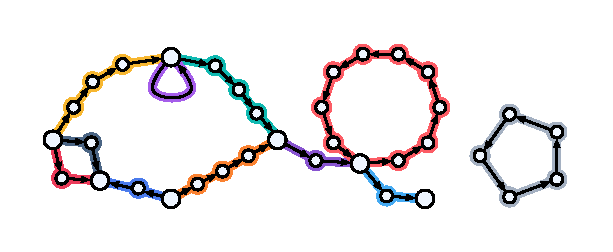
\includegraphics[width=.6\linewidth]{fig/minimization-crpq/segments.pdf}
	}
	\hfill%
	\subfloat[The "segment graph" of $\gamma$.]{%
		\AP\label{fig:segment-graph}%
		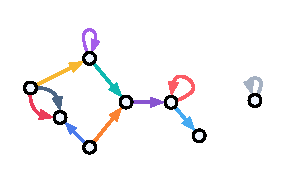
\includegraphics[width=.38\linewidth]{fig/minimization-crpq/segment-graph.pdf}
	}
	\caption{"Segments" and "segment graph" of a "CRPQ" $\gamma$.}
\end{figure}

\begin{fact}
	\AP\label{fact:partition-into-segments}
	The "segments"---seen as sets of "atoms"---of $\gamma$ form a partition on its set of "atoms".
\end{fact}

See \Cref{fig:segments} for an example of a decomposition into "segments".
Note that each "segment" is "incident@@segment" to either zero "external variable" (isolated cycles),
to one (non-isolated cycles) or to two (non-cycles).
We denote by \AP$\intro*\nbseg{\gamma}$ the number of "segments" of a "CRPQ" $\gamma$,
and we extend this notation to "UCRPQs" by letting $\nbseg{\Gamma} \defeq
\max_{\gamma \in \Gamma}{\nbseg{\gamma}}$. By \Cref{fact:partition-into-segments}, $\nbseg{\Gamma}\leq \nbatoms{\Gamma}$ always holds.

\subsection{Necessary Conditions: Contractions and Redundancy}

\paragraph{Contractions.}
One simple (and tractable) way to make a query smaller is to `contract' any two consecutive atoms in a path with just one atom having the concatenation of the languages.
A "CRPQ" $\gamma$ is \AP""fully contracted"" if it cannot be "contracted".
In other words, $\gamma$ is "fully contracted" "iff" $\nbseg{\gamma} = \nbatoms{\gamma}$.
A "contraction" of a "UCRPQ" is a "contraction" of a "CRPQ" therein (obtaining the "UCRPQ" where one "CRPQ" $\gamma$ was replaced by a "contraction" of $\gamma$). A "UCRPQ" is then \reintro{fully contracted} if each "CRPQ" therein is "fully contracted".

\begin{fact}
	\AP\label{fact:produce-fully-contracted}
	"Contractions" preserve "semantic equivalence". Further, from a "UCRPQ" $\Gamma$ one can produce, in polynomial time, an "equivalent" one that is "fully contracted" with $\nbseg{\Gamma}$ "atoms".
\end{fact}

In particular, if a "UCRPQ" $\Gamma$ is "minimal" then $\Gamma$ is "fully contracted" and $\nbseg{\Gamma} = \nbatoms{\Gamma}$; in other words, $\nbseg{\Gamma}$ is an upper bound on the number of atoms of the "minimal" equivalent query.

\paragraph{Redundancy}
Another way to reduce the number of atoms of a query is to remove any \AP""redundant atom"", that is, any "atom" whose removal results in an "equivalent" query. 
When there are no such redundant atoms, we say that the query is \reintro{non-redundant}.
However, this is a more difficult problem, since it involves testing for query equivalence, an "ExpSpace"-complete problem.

\begin{proposition}
	\AP\label{prop:lowerbound-non-redundant}
	% The problem of 
	Testing whether a "(U)CRPQ@UCRPQ" is "non-redundant" is "ExpSpace"-complete.
\end{proposition}

\begin{proof}
	The upper bound is trivial: for every "atom" we remove it and check "equivalence".
	
	\todo{move this! this is forward ref}
	For the lower bound, we use the construction of \Cref{prop:variation-figueira} for containment. Let $\delta() 
	\defeq x' \atom{K} y' \land \bigwedge_i x \atom{L_i} y$ be the "disjoint conjunction" of $\gamma_1()$ and $\gamma_2()$ as defined in \Cref{prop:variation-figueira}.
	We first strengthen the construction to ensure the following two properties:
	\begin{enumerate}
		\item \textbf{$K$ cannot be mapped inside any $L_i$}: There is no word of $K$ which appears as factor of a word from some $L_i$. For this, it suffices to add a special letter at the beginning and the end of every word of $K$ which is not in any of the $L_i$'s. That is, we can define a new $K^{\textit{new}} \defeq \# \cdot K^{\textit{old}} \cdot \#$ for a new symbol $\#$.
		\item \textbf{For every $j$ there is $w_j \in L_j$ such that $w_j \not\in L_i$ for every $i \neq j$}: it suffices to add a special word ("eg" using a new alphabet letter) to each $L_i$. For example, we can define $L_{i}^{\textit{new}} \defeq L_{i}^\textit{old} \cup \set{@_i}$, where $@_i$ is a fresh alphabet letter.
	\end{enumerate}
	It is easy to see that these modifications preserve all the properties needed for the "containment problem" to still be "ExpSpace"-hard.
	
	We show that $\delta()$ is "non-redundant" "iff" $x' \atom{K} y' \contained \bigwedge_i x \atom{L_i} y$.
	
	\proofcase{$K$ cannot be removed.} We first show that removing the atom $x' \atom{K} y'$ from $\delta()$ results in a non-"equivalent" query $\delta'()$. Indeed, if it is removed then for any expansion of $\delta'()$ there will not be any word from $K$ that can be used to map into the expansion due to the first point above.

	\proofcase{If some $L_j$ is redundant, then containment holds.} Consider the result $\delta'()$ of removing an atom $x \atom{L_j} y$ from $\delta()$. Consider all the expansions of $\delta'()$ that choose $w_i$---defined in the second point above---as the "atom expansion" for $L_i$ for every $i \neq j$. It follows that for any such expansion there must be an expansion of $\delta()$ that maps necessarily $x \atom{L_j} y$ to the "atom expansion" of $x' \atom{K} y'$ in $\delta'()$. Otherwise, we would be mapping some word of $L_j$ to some $w_i$ with $i\neq j$, which we know it is not possible due to the second point above.
	This means that $x' \atom{K} y' \contained \bigwedge_i x \atom{L_i} y$.

	\proofcase{If containment holds, then all $L_i$'s redundant.} Finally, observe that if $x' \atom{K} y' \contained \bigwedge_i x \atom{L_i} y$ then the query is "equivalent" to $x' \atom{K} y'$.

	Overall, we obtained that the following are equivalent:
	\begin{enumerate}[label=\roman*.]
		\item $\delta()$ is "redundant",
		\item an atom $x \atom{L_i} y$ of $\delta()$ is "redundant",
		\item the containment $x' \atom{K} y' \contained \bigwedge_i x \atom{L_i} y$ holds,
		\item all atoms $x \atom{L_i} y$ of $\delta()$ are "redundant".\qedhere
	\end{enumerate}
\end{proof}

While in the case of "conjunctive queries" "non-redundancy" is the same as "minimality", for "CRPQs" and "UCRPQs" this is not the case, even if the query is "fully contracted". 

\begin{proposition}
	There are "fully contracted" "non-redundant" "CRPQs" which are not "minimal".
\end{proposition}

\begin{proof}
	\begin{figure}
		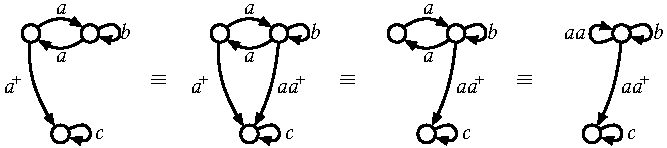
\includegraphics[scale=.8]{fig/minimization-crpq/ex-equiv-queries.pdf}
		\caption{"Equivalent" "CRPQs". The leftmost query is "fully contracted", "non-redundant" and not "minimal", since it is "equivalent" to the rightmost query.}
		\AP\label{fig:ex-equiv-queries}
	\end{figure}
	\Cref{fig:ex-equiv-queries} contains a simple witnessing example. It is trivial to see that the "CRPQs" in the figure are all "equivalent" and that the leftmost query is "non-redundant" and "fully contracted". However, it is not "minimal" since it is "equivalent" to the rightmost "CRPQ".
\end{proof}

\subsection{A Sufficient Condition: Strong Minimality}

We have seen some sound ways to reduce the size of queries. But how can we ensure that a query is actually minimal? Here we give a theoretical tool which can ensure this by means of finding some "expansion" which is a witness for the query to have ``many atoms''. We call this "strong minimality".

Say that an "expansion" $\anexpansion$ of a "UCRPQ" $\Gamma$ is \AP""hom-minimal"" when, for every "expansion" $\anexpansion'$ of $\Gamma$, if $\anexpansion' \homto \anexpansion$ then $\anexpansion'$ and $\anexpansion$ are "hom-equivalent". 

A "UCRPQ" $\Gamma$ is \AP""strongly minimal"" if 
it has a "hom-minimal" "expansion" $\anexpansion \in \Exp(\Gamma)$ "st" $\nbseg{\core(\anexpansion)} = \nbatoms{\Gamma}$. We will next show that this is a sufficient condition for minimality.

Informally, the segment graph $\reintro*\seggraph(\gamma)$ of a "CRPQ" $\gamma$ is the directed multigraph obtained by replacing "segments" of $\gamma$ with edges in its "underlying graph", as illustrated in \Cref{fig:segment-graph}. The main motivation behind the notion of "segments" is 
that it is essentially dual to the notion of "atom refinements".

\begin{definition}
	\AP\label{defn:segmentgraph}
	Given a "CRPQ" $\gamma$, we define its \AP""segment graph"" $\intro*\seggraph(\gamma)$
	to be the directed multigraph defined by:
	\begin{itemize}
		\item every "external variable" of $\gamma$ is a vertex of $\seggraph(\gamma)$,
			and moreover, for every "cyclic segment" $\sigma$
			that is not "incident@@segment" to any "external variable", we create a new variable
			$x_\sigma$;
		\item for every "cyclic segment" $\sigma$, we have a self-loop around $x_{\sigma}$,
			and for any "external variable" $x$ and $y$ of $\gamma$, we have an edge
			from $x$ to $y$ in $\seggraph(\gamma)$ for any "segment" starting at $x$ and
			ending at $y$.
	\end{itemize}
\end{definition}

\begin{fact}
	\AP\label{fact:segment-graph-is-contraction}
	The "segment graph" of $\gamma$ can always be obtained from its "underlying
	graph" by "contracting internal variables". 
\end{fact}

A \AP""minor"" of a graph is any graph that can be obtained by removing
edges, removing vertices---and their adjacent edges---, and \AP""contracting edges""---meaning that we identify the two endpoints of the edge and remove the edge from the graph.%
\footnote{This definition is a trivial generalization of the notion of minors for undirected graphs.} Moreover, we say that a "class of CRPQs" is ""minor-closed"" when, for every
"query@@CRPQ" is the class, any other "query@@CRPQ" whose "underlying graph@@dir" 
is a "minor" of the "underlying graph@@dir" of the first query must also
belong to the class.

\begin{figure}
	\centering
	\subfloat[A "CRPQ" $\gamma$.]{%
		\AP\label{fig:example-crpq}%
		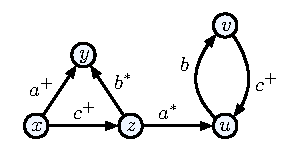
\includegraphics[width=.41\linewidth]{fig/minimization-crpq/example-crpq.pdf}
	}
	\hfill
	\subfloat[An "expansion" $\xi$ of $\gamma$, together with its "segments".]{%
		\AP\label{fig:segments-expansion}%	
		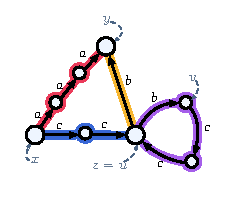
\includegraphics[width=.32\linewidth]{fig/minimization-crpq/segments-expansion.pdf}
	}
	\hfill
	\subfloat[The "segment graph" of $\xi$.]{%
		\AP\label{fig:segment-graph-expansion}%
		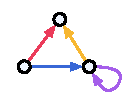
\includegraphics[width=.21\linewidth]{fig/minimization-crpq/segment-graph-expansion.pdf}
	}
	\caption{%
	\AP\label{fig:seggraph-of-expansion}
		Illustration of \Cref{prop:seggraph-of-expansion}:
		\Cref{fig:segment-graph-expansion} can be obtained as a "minor" of 
		\Cref{fig:example-crpq}.
	}
\end{figure}

\begin{proposition}
	\AP\label{prop:seggraph-of-expansion}
	Let $\gamma$ be a "CRPQ" and $\anexpansion$ be an "expansion" of $\gamma$.
	Then $\seggraph(\anexpansion)$ is a "minor" of
	the "underlying graph" of $\gamma$.%
	\footnote{In general, $\seggraph(\anexpansion)$
	can be obtained by "contracting edges", but there are some degenerate cases where we must
	remove some vertices, for instance when considering the "expansion" of $x \atom{a^*} x$
	associated with the empty word. This is an artefact of our choice to disallow isolated variables
	in "CRPQs".}
\end{proposition}

In particular, $\nbseg{\anexpansion} \leq \nbatoms{\gamma}$.
See \Cref{fig:seggraph-of-expansion} for an example.

\begin{proof}
	The "underlying graph" of $\anexpansion$ is obtained from
	the "underlying graph" of $\gamma$ by:
	\begin{enumerate}
		\item contracting some edges---corresponding to "atom refinements"
			for the word $\varepsilon$,
				 \item potentially removing isolated vertices,\footnote{This can happen "eg" in the "atom refinement" of $x \atom{a^*} x$ when dealing with the empty word.} and
		\item "refining" some edges---corresponding to "atom refinements"
			for words of length at least 2.
	\end{enumerate}
	Let $G'$ be the "underlying graph" of $\gamma$ to which we applied 
	all operation of type (1) and (2). By construction,
	$G'$ is a "minor" of $\underlying{\gamma}$.
	Notice then that if $H$ is a graph obtained by "refining" one edge of $G'$,
	then $\seggraph(H)$ and $\seggraph(G')$ are isomorphic.
	By trivial induction, it follows that $\seggraph(\anexpansion)$
	is isomorphic to $\seggraph(G')$.
	In turn, by \Cref{fact:segment-graph-is-contraction}, $\seggraph(G')$
	is an "edge contraction" of $G'$, which concludes the proof
	since the latter is a "minor" of $\underlying{\gamma}$.
\end{proof}

The next proposition provides a helpful tool to prove lower bounds on the
number of "atoms"---but also on the structure---required to express a query.
\AP\phantomintro{Semantical Structure}

\begin{theorem}[\reintro{Semantical Structure}]
	\AP\label{thm:structure-theorem}
	Let $\Gamma$ be a "UCRPQ".
	Let $\anexpansion$ be a "hom-minimal" "expansion" of $\Gamma$,
	and $\Delta$ be any "UCRPQ" "equivalent" to $\Gamma$.
	Then there exists some $\delta \in \Delta$ "st" the "segment graph" $\seggraph(\core(\anexpansion))$
	of the "core" of $\anexpansion$ is a "minor" of the "underlying graph" of $\delta$. 
\end{theorem}

\begin{proof}
	Let $\Gamma$ be a fixed "UCRPQ", and let $\Delta$ be a "equivalent" "UCRPQ".
	Let $\anexpansion_\Gamma$ be a "hom-minimal" "expansion" of $\Gamma$.
	Since $\Gamma \contained \Delta$, there exists an "expansion" $\anexpansion_\Delta$ of $\Delta$
	"st" $\anexpansion_\Delta \homto \anexpansion_\Gamma$. Likewise, since $\Delta \contained \Gamma$, there exists an "expansion" $\anexpansion'_\Gamma \in \Exp(\Gamma)$ "st"
	$\anexpansion'_\Gamma \homto \anexpansion_\Delta$. Overall, we have
	$\anexpansion'_\Gamma \homto \anexpansion_\Gamma$ and so,
	by "hom-minimality" of $\anexpansion_\Gamma$, it is "hom-equivalent" to $\anexpansion'_\Gamma$. In turn, this implies that $\anexpansion_\Delta$ is "hom-equivalent" to $\anexpansion_\Gamma$, 
	and thus there exists an "embedding" of
	$\core(\anexpansion_\Gamma)$ into $\anexpansion_\Delta$.
	Note moreover that such an "embedding" must send variables of
	in-degree 0 (resp. out-degree 0) to nodes of in-degree 0 (resp. out-degree 0)
	and so by \Cref{coro:embedding-segments},
	there is an "embedding" from $\seggraph(\core(\anexpansion_\Gamma))$
	into $\seggraph(\anexpansion_\Delta)$.
	Letting $\delta$ be the "disjunct" of $\Delta$ of which $\anexpansion_\Delta$ is an "expansion",
	\Cref{prop:seggraph-of-expansion} implies that $\seggraph(\anexpansion_\Delta)$ is a
	"minor" of the "underlying graph" of $\delta$.
	Hence, $\seggraph(\core(\anexpansion_\Gamma))$ is a subgraph of a "minor", and hence a "minor", of the "underlying graph" of $\delta$.
\end{proof}

\begin{corollary}[of \Cref{thm:structure-theorem}]
	\AP\label{coro:strong-min}
	Every "strongly minimal" "UCRPQ" is "minimal".
\end{corollary}

\begin{proof}
	The number of edges of $\seggraph(\core(\anexpansion))$ equals $\nbseg{\core(\anexpansion)}$, and a "minor" can only decrease the number of edges.
\end{proof}

In fact, it can be seen that the assumption that $\anexpansion$ is "hom-minimal" in
\Cref{thm:structure-theorem} is necessary as otherwise the statement would be false (see \Cref{rk:structure-theorem} for details).
%
Also, note in particular that \Cref{thm:structure-theorem} implies
$\nbseg{\core(\anexpansion)} \leq \nbatoms{\Delta}$. 
But it can also be used to obtain lower bounds on, for instance,
the tree-width of $\Delta$, and hence the one-way semantic tree-width\footnote{Defined in
\cite[\S 1, p. 7]{FigueiraMorvan2025SemanticTreeWidthLMCS}.} of $\Gamma$, 
or more generally to prove that $\Gamma$ cannot be "equivalent" to a "UCRPQ" whose
underlying graphs all belong to a "minor"-closed class of graphs.

\begin{proposition}
	\AP\label{prop:union-segments}
	Let $\gamma$ be a "CRPQ".
	The set of "atoms" of any path $x_0 \atom{a_1} \cdots \atom{a_n} x_n$ of $\gamma$
	where either $x_0 = x_n$ or where both $x_0$ and $x_n$ are "external" 
	is a finite union of "segments" of $\gamma$.
\end{proposition}
	
\begin{proof}
	The statement deals with the set of "atoms" of the path---and not the path itself---,
	so "wlog", up to a circular permutation of the path, we assume that (\adforn{75})
	if $x_0 = x_n$
	then either $x_0$ and $x_n$ are "external", or all $x_i$'s ($i \in \lBrack 1,n-1\rBrack$)
	are "internal".

	We prove the statement by induction on the length of the path.
	We identify three cases:
	\begin{enumerate}
		\item each $x_i$ ($i \in \lBrack 1,n-1 \rBrack$) is both
			"internal" and distinct from all $x_j$'s ($j\in \lBrack 0,n\rBrack$);
		\item $x_0$ and $x_n$ are "external" and there exists
			$i \in \lBrack 1,n-1 \rBrack$ "st" $x_i$ is "external";
		\item $x_0 = x_n$ and there exists $k \in \lBrack 1,n-1 \rBrack$
					"st" $x_k = x_0 \mathrel{(=} x_n)$.
	\end{enumerate}
	Next, we show that this covers all possible cases.

	If we are not in the first case, then either some
	$x_i$ ($i \in \lBrack 1,n-1 \rBrack$) is "external" or is equal to some $x_j$ ($j\in \lBrack 0,n\rBrack$). For the former, by (\adforn{75}) we get that $x_0$ and $x_n$ are necessarily
	"external", and we fall in case 2.
	
	For the former, we know that all $x_i$'s 
	($i \in \lBrack 1,n-1 \rBrack$) are "internal", and there exists $i \in \lBrack 1,n-1 \rBrack$
	and $j\in \lBrack 0,n\rBrack$ "st" $x_i = x_j$. Up to renaming the variables, we get 
	that $i<j$ and $(i,j) \neq (0,n)$. 
	Recall that all $x_k$'s ($k \in \lBrack 1,n-1 \rBrack$) are "internal",
	and so from $x_i = x_j$ we get by trivial induction that $x_0 = x_{j-i}$.
	In particular, $x_0$ must be "internal" and so $x_0 = x_n$.
	Letting $k \defeq j-i$ we have $k \in \lBrack 1,n-1 \rBrack$ "st" 
	$x_k = x_0 = x_n$, and so we are in case 3.

	We can now proceed with the induction.
	\begin{enumerate}
		\item For the base case, we have a path where each $x_i$ ($i \in \lBrack 1,n-1 \rBrack$)
			is both "internal" and distinct from all $x_j$'s ($j\in \lBrack 0,n\rBrack$).
			By definition this path is a "segment".
		\item In the second case, $x_0$ and $x_n$ are "external", and there exists
			some $i \in \lBrack 1,n-1 \rBrack$
			"st" $x_i$ is "external". We use the induction hypothesis on the paths
			$x_0 \atom{a_1} \cdots \atom{a_i} x_i$ and $x_i \atom{a_{i+1}} \cdots \atom{a_n} x_n$
			and the conclusion follows.
		\item In the last case, there exists $k \in \lBrack 1,n-1 \rBrack$
				"st" $x_0 = x_k = x_n$, and the conclusion follows from applying the
				induction on $x_0 \atom{a_1} \cdots \atom{a_k} x_k$ and
				$x_k \atom{a_{k+1}} \cdots \atom{a_n} x_n$.
	\end{enumerate}
	This concludes the induction and the proof.
\end{proof}

\begin{lemma}
	\AP\label{lemma:hom-segments}
	Let $\gamma,\delta$ be "CRPQs".
	If $f\colon \delta \to \gamma$ is a "homomorphism" that sends "external variables"
	of $\delta$ on "external variables" of $\gamma$, then there is a
	function from nodes of $\seggraph(\delta)$ to nodes of $\seggraph(\gamma)$  
	that sends an edge of $\seggraph(\delta)$ to a path of $\seggraph(\gamma)$.
\end{lemma}

\begin{proof}
	By \Cref{prop:union-segments}, the image
	$f[\sigma]$ by $f$ of any "segment" $\sigma$ of $\delta$ is a union of
	"segments" of $\gamma$.
\end{proof}

\begin{corollary}
	\AP\label{coro:embedding-segments}
	Let $\gamma, \delta$ be two "CRPQs" such that there is an "embedding" from $\delta$ to $\gamma$
	"st" every node of in-degree 0 (resp. out-degree 0) is sent on a node of in-degree 0
	(resp. out-degree 0). 
	Then $\seggraph(\delta)$ is a "minor" of $\seggraph(\gamma)$.
\end{corollary}

\begin{proof}
	Let $f\colon \delta \to \gamma$ be such an "embedding".
	\begin{claim}
		\AP\label{claim:hom-preserves-non-internality}
		If $x \in \delta$ is "external", then $f(x)$ is "external".
	\end{claim}
	Indeed, if $x$ has in-degree at least 2, or out-degree at least 2,
	so does $f(x)$ since $f$ is an "embedding".
	Otherwise, either $x$ has either in-degree 0 or out-degree 0,
	and so does $f(x)$ using the assumption we made on $f$.

	We then use \Cref{lemma:hom-segments}.
	Note that since $f$ is an "embedding", the segments of $\gamma$ occurring in
	$f[\sigma]$ must be distinct from the segments occurring in $f[\sigma']$
	for any "segment" $\sigma' \neq \sigma$.
	Overall, we have an injective map from nodes of $\seggraph(\delta)$ 
	to nodes of $\seggraph(\gamma)$, which sends an edge to a path,
	and moreover these paths are pairwise disjoint.
	This shows that $\seggraph(\delta)$ is a "minor" of $\seggraph(\gamma)$.
\end{proof}

\begin{remark}
	\AP\label{rk:structure-theorem}
	Note that the assumption that $\anexpansion$ is "hom-minimal" in
	\Cref{thm:structure-theorem} is necessary: consider the "CRPQ"
	$\gamma(x,y) \defeq x \atom{a^+} y \land x \atom{(aa)^+} y$.
	For $n,m \in \Np$, let $\anexpansion_{n,m}(x,y) \defeq x \atom{a^n} y \land x \atom{a^{2m}} y$.
	There are two cases:
	\begin{enumerate}
		\item \AP\label{rk:structure-theorem:1} If $n \neq 2m$, then $\nbseg{\core(\anexpansion_{n,m})} = 2$
			but $\anexpansion_{n,m}$ is not "hom-minimal" since $\anexpansion_{2m,m} \homto \anexpansion_{n,m}$ but $\anexpansion_{n,m} \nothomto \anexpansion_{2m,m}$.
		\item If $n = 2m$, then $\nbseg{\core(\anexpansion_{n,m})} = 1$
		and $\anexpansion_{n,m}$ is "hom-minimal".
	\end{enumerate}
	Hence, using \Cref{thm:structure-theorem}, we can only get a lower bound of
	one "atom" (and not two) on the size of any "UCRPQ" "equivalent" to $\gamma(x,y)$,
	which is consistent with the fact that $\gamma(x,y) \semequiv \gamma'(x,y)$
	where $\gamma'(x,y) \defeq x \atom{(aa)^+} y$.
	If \Cref{thm:structure-theorem} would allow for non "hom-minimal" queries we would obtain, by \Cref{rk:structure-theorem:1} a lower bound of 2 "atoms", which is false.
\end{remark}

However, this is a sound but unsurprisingly not a complete characterization of "minimality".

\begin{proposition}
	There are "minimal" "(U)CRPQs@CRPQ" which are not "strongly minimal". 
\end{proposition}

\begin{proof}
	The "Boolean" "CRPQ" $\gamma() = x \atom{a^+} x$. Since it has one atom, it must be "minimal", but it has no "hom-minimal" "expansions".
\end{proof}

Finally, we show that checking strong minimality is at least as hard as checking containment.

\begin{proposition}
	\AP\label{prop:lowerbound-strong-minimality}
	Testing whether a "(U)CRPQ@UCRPQ" is "strongly minimal" is "ExpSpace"-hard.
\end{proposition}

\begin{proof}
	We use the same reduction as in \Cref{prop:lowerbound-non-redundant}.
	If $\delta$ is "strongly minimal", then it is "minimal", and so it is
	"non-redundant", and hence
	by the proof of \Cref{prop:lowerbound-non-redundant},
	$x' \atom{K} y' \notcontained \bigwedge_i x \atom{L_i} y$.
	
	We prove the converse implication: assume that
		$x' \atom{K} y' \notcontained \bigwedge_i x \atom{L_i} y$.
	Then there exists $\#u\# \in K$ "st" $x' \atom{\#u\#} y'$
	does not "satisfy@@db" $\bigwedge_i x \atom{L_i} y$.
	Consider the "expansion" $\anexpansion$ obtained by replacing $K$ with $\#u\#$, and replacing 
	$L_i$ with $@_i$ for each $i$.
	Then $\anexpansion$ is a "core" because of the fresh letters $\#$ and $@_i$.
	Moreover, we claim that it has to be "hom-minimal".
	Indeed, assume that some other "expansion" $\anexpansion'$ is "st" $\anexpansion'\homto \anexpansion$.
	Then because of $\#$, the "atom expansion" of $x' \atom{K} y'$ in $\anexpansion'$ 
	must be mapped on $x' \atom{\# u \#} y'$ in $\anexpansion$.
	Then, by definition of $u$, the "atom expansions" of $\bigwedge_i x \atom{L_i} y$
	cannot be mapped on $x' \atom{\# u \#} y'$, and so they must be mapped on
	$\bigwedge_i x \atom{@_i} y$, and hence $\anexpansion' = \anexpansion$.
	Hence, this shows that $\delta$ is "strongly minimal".
	Overall, we showed that $x' \atom{K} y' \notcontained \bigwedge_i x \atom{L_i} y$
	"iff" $\delta$ is "strongly minimal", which concludes our reduction.
\end{proof}